\documentclass{article}
\usepackage[utf8]{inputenc}
\usepackage{graphicx}
\usepackage{amsmath}
\usepackage{amsfonts}
\usepackage{amssymb}
\usepackage{tikz}
\newcommand{\norm}[1]{\left\lVert#1\right\rVert}
\def\layersep{2.5cm}

\title{Notes on Neural Networks}
\author{Trevin Gandhi}
\date{2015}

\begin{document}

\maketitle

\section{The Neuron}
	Let us first consider a neuron, the basic building block of nervous systems. \\
	\includegraphics[width=\textwidth]{neuron}
	There are quite a few labels in this diagram, but let's only consider the axon and dendrites for now. The dendrite is the part of the neuron that receives signals from other neurons. This signal is in the form of an electrical impulse known as the \textit{action potential}, which enters the neuron through the sodium-potassium pumps in the neuron's membrane. If this action potential is large enough, it gets transmitted through the neuron and down the axon in a wave-like manner. The action potential then continues out of the axon and on to other neurons. From this description, we can pull away 3 key features of a neuron: \\
	\begin{enumerate}
		\item Synaptic Weights - The action potential won't be propagated through the neuron unless it is large enough.
		\item Cumulative Stimulus - The action potentials transmitted from all nearby neurons can be picked up by the dendrites. Their action potentials will simply be summed into one total action potential.
		\item All or Nothing - If an action potential is not large enough to get propagated through the neuron, nothing will get transmitted - it is an all or nothing situation.
	\end{enumerate}
	Based on these, we can begin modeling these neurons with our own artificial ones that feature the same properties.

\section{Perceptrons}
	A ``perceptron'' is a very basic model of a neuron. It inherently has its own vector of weights $w$, where each element represents the weight associated with the corresponding decision.  A perceptron also has a bias, $b$, used to make the decision. The perceptron takes as input a binary vector $x$ representing the conditions relevant for each decision. Then the output of the perceptron, which is a single ``yes'' or ``no'' is as follows:
	\begin{equation}
	\text{output } = \begin{cases} 0 &\mbox{if } w \cdot x + b \leq 0 \\
					          1 &\mbox{if } w \cdot x + b > 0 \end{cases}
	\end{equation}

	Cool things: You can layer perceptrons for more complex decision making. You can also use perceptrons to imitate logic gates.

\section{Sigmoid Neurons}
	Sigmoid neurons are similar to perceptrons in that they take in a vector $x$ as input, have weights and a bias, and produce an output decision. The key conceptual difference, however, is that sigmoid neurons are designed so that small changes in their weights and bias only have small effects on their output decision. This allows sigmoid neurons to be continuously ``fine-tuned'' towards optimal decision-making. 

	To manifest this conceptual change, sigmoid neurons can take a vector $x$ where each element is in the interval $[0, 1]$, not just from the set ${0, 1}$ like it was with perceptrons. Additionally, sigmoid neurons do not output a binary decision - they output a sigmoid (or logistic) function. \\
	The basic sigmoid function is defined by:
	\begin{equation}
		\sigma (z) \equiv \frac{1}{1 + e^{-z}}
	\end{equation}
	meaning that a sigmoid neuron would output:
	\begin{equation}
		\text{output } = \frac{1}{1 + e^{-\sum_{j}w_j x_j - b}}
	\end{equation}
	and in vectorized form:
	\begin{equation}
		\text{output } = \frac{1}{1 + e^{- (w \cdot x) - b}}
	\end{equation}

	Because the logistic function is a smooth function ranging from 0 to 1 (as opposed to a step function), it results in small changes being made to the output when small changes are made to the weights or bias. The change in output, $\Delta \text{output}$,  can be approximated by:
	\begin{equation}
		\Delta \text{output} \approx \sum_{j} \frac{\partial \text{output}}{\partial w_j} \Delta w_j + \frac{\partial \text{output}}{\partial b} \Delta b
	\end{equation}

	\subsection{Exercises}
		\begin{enumerate}
			\item
				Question: Suppose we take all the weights and biases in a network of perceptrons, and multiply them by a positive constant, $c>0$. Show that the behavior of the network doesn't change. \\
				Answer: The output for a perceptron is:
				\begin{equation*}
					\text{output } = \begin{cases} 0 &\mbox{if } w \cdot x + b \leq 0 \\
								          1 &\mbox{if } w \cdot x + b > 0 \end{cases}
				\end{equation*}
				and if scaled by $c$,
				\begin{equation*}
					\text{output } = \begin{cases} 0 &\mbox{if } c(w \cdot x + b) \leq 0 \\
								          1 &\mbox{if } c(w \cdot x + b) > 0 \end{cases}
				\end{equation*}
				and because $c > 0$, we can say
				\begin{equation*}
					\text{output } = \begin{cases} 0 &\mbox{if } w \cdot x + b \leq 0 \\
								          1 &\mbox{if } w \cdot x + b > 0 \end{cases}
				\end{equation*}
				and thus the behavior of the perceptron network does not change, as each perceptron is outputting the same thing as it did pre-scaling. \\

		\item
			Question: Suppose we have the same setup as the last problem - a network of perceptrons. Suppose also that the overall input to the network of perceptrons has been chosen. We won't need the actual input value, we just need the input to have been fixed. Suppose the weights and biases are such that $w\cdot x+b \neq 0$ for the input $x$ to any particular perceptron in the network. Now replace all the perceptrons in the network by sigmoid neurons, and multiply the weights and biases by a positive constant $c>0$. Show that in the limit as $c \rightarrow \infty$ the behavior of this network of sigmoid neurons is exactly the same as the network of perceptrons. How can this fail when $w\cdot x+b=0$ for one of the perceptrons? \\
			Answer: The output of a sigmoid neuron is given by: \\
			\begin{equation*}
				\text{output } = \frac{1}{1 + e^{- (w \cdot x) - b}}
			\end{equation*}
			and thus the output of the scaled sigmoid neuron is:
			\begin{equation*}
				\text{output } = \frac{1}{1 + e^{-c(w \cdot x + b)}}
			\end{equation*}
			Therefore, when we take $\lim_{c \to \infty} e^{-c(w \cdot x + b)}$, we can rewrite that as $e^{-\infty (w \cdot x + b)}$. We now have two cases: \\
			1) if $w \cdot x + b < 0$, then the negatives cancel and the term becomes $\infty$. Thus, the output can be rewritten as: 
			\begin{equation*}
				\text{output } = \frac{1}{1 + \infty} \approx 0
			\end{equation*}
			just like with a perceptron. \\
			2) if $w \cdot x + b > 0$, then the term becomes $\approx 0$. Thus, the output can be rewritten as: 
			\begin{equation*}
				\text{output } = \frac{1}{1 + 0} = 1
			\end{equation*}
			again, just like with a perceptron. \\
			And now we can see how this fails if $w \cdot x + b = 0$, because then the output becomes:
			\begin{equation*}
				\text{output } = \frac{1}{1 + 1} = \frac{1}{2}
			\end{equation*}
			which is not part of the set ${0, 1}$ that a perceptron draws its output from.
		\end{enumerate}

\section{The architecture of neural networks}
	In a neural network, the leftmost layer is called the input layer (containing \textit{input neurons}), the middle layers are called the hidden layers, and the rightmost layer is called the output layer (containing \textit{output neurons}).

	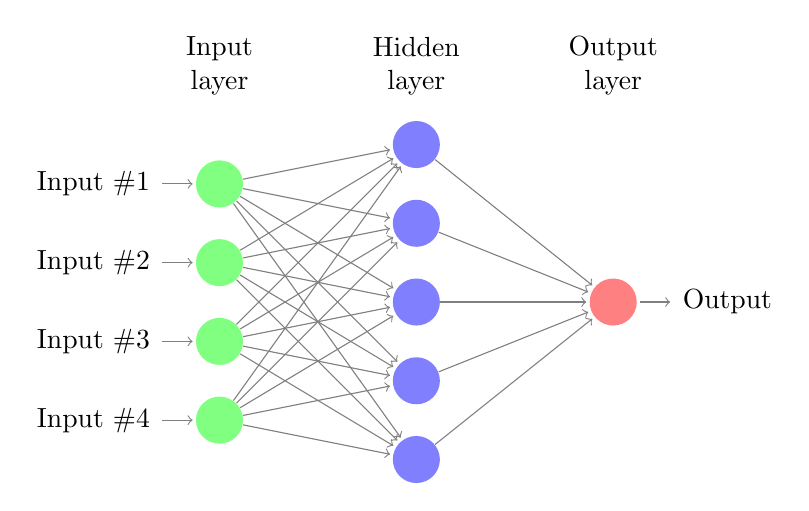
\begin{tikzpicture}[shorten >=1pt,->,draw=black!50, node distance=\layersep]
	    \tikzstyle{every pin edge}=[<-,shorten <=1pt]
	    \tikzstyle{neuron}=[circle,fill=black!25,minimum size=17pt,inner sep=0pt]
	    \tikzstyle{input neuron}=[neuron, fill=green!50];
	    \tikzstyle{output neuron}=[neuron, fill=red!50];
	    \tikzstyle{hidden neuron}=[neuron, fill=blue!50];
	    \tikzstyle{annot} = [text width=4em, text centered]

	    % Draw the input layer nodes
	    \foreach \name / \y in {1,...,4}
	    % This is the same as writing \foreach \name / \y in {1/1,2/2,3/3,4/4}
	        \node[input neuron, pin=left:Input \#\y] (I-\name) at (0,-\y) {};

	    % Draw the hidden layer nodes
	    \foreach \name / \y in {1,...,5}
	        \path[yshift=0.5cm]
	            node[hidden neuron] (H-\name) at (\layersep,-\y cm) {};

	    % Draw the output layer node
	    \node[output neuron,pin={[pin edge={->}]right:Output}, right of=H-3] (O) {};

	    % Connect every node in the input layer with every node in the
	    % hidden layer.
	    \foreach \source in {1,...,4}
	        \foreach \dest in {1,...,5}
	            \path (I-\source) edge (H-\dest);

	    % Connect every node in the hidden layer with the output layer
	    \foreach \source in {1,...,5}
	        \path (H-\source) edge (O);

	    % Annotate the layers
	    \node[annot,above of=H-1, node distance=1cm] (hl) {Hidden layer};
	    \node[annot,left of=hl] {Input layer};
	    \node[annot,right of=hl] {Output layer};
	\end{tikzpicture}

\section{A simple network to classify handwritten digits}
	The input layer consists of 784 neurons, each representing a pixel of the 28x28 pixel image of a handwritten digit. The hidden layer consists of a currently undecided $n$ neurons, and the output layer contains 10 neurons - each representing what number the neural network has classified the digit as (i.e. the first output neuron firing would say that the digit is a 0).

\section{Gradient Descent}
	We can define a cost function $C(w, b)$ that represents how close our approximation (what the neural network is outputting) is to the real deal. A simple quadratic cost function is: 
	\begin{equation}
		C(w, b) \equiv \frac{1}{2n} \sum_{x} \norm{y(x) - a}^2
	\end{equation}
	In this case, y(x) is the function we are trying to approximate and $a$ is our approximation (the output). \\
	Now, to optimize our neural network, we clearly want to minimize our cost function. We can do this with a method called gradient descent, where we iteratively approach the minimum of a function. Recall the gradient function from multi-variable calculus:
	\begin{equation}
		\nabla F(x_1, x_2, \dots, x_n) = (\frac{\partial F}{\partial x_1}, \frac{\partial F}{\partial x_2}, \dots, \frac{\partial F}{\partial x_n})^{T}
	\end{equation}
	We can use this gradient function to approximate $\Delta F$:
	\begin{equation}
		\Delta F \approx \nabla F \cdot \Delta x
	\end{equation}
	To find the minimum, we can simply update $x$ based on the negative gradient:
	\begin{equation}
		\Delta v = -\eta \nabla F
	\end{equation}
	where $\eta$ is the learning rate. To put this back in terms of our cost function $C$, we can say that: \\
	\begin{equation}
		\Delta w_k = -\eta * \frac{\partial C}{\partial w_k}
	\end{equation}
	\begin{equation}
		\Delta b_l = -\eta * \frac{\partial C}{\partial b_l}
	\end{equation}
	However, there is an inherent flaw in this approach: because $\nabla C$ is defined as:
	\begin{equation*}
		\nabla C = \frac{1}{n} sum_{x} \nabla C_x
	\end{equation*}
	$\nabla C_x$ would need to be computed for each training input $x$ - which can be computationally inefficient when $x$ is very large. \\
	Thus, we have the idea of \textit{stochastic gradient descent}, which randomly selects a \textit{mini-batch} of training inputs to calculate an approximation of $\nabla C$. If $m$ denotes the size of the mini-batch and $n$ the number of training inputs, then we know:
	\begin{equation}
		\lim_{m \to n} \frac{sum_{j=1}^{m} \nabla C_{X_j}}{m} = \frac{\sum_x \nabla C_x}{n} = \nabla C
	\end{equation}
	The process works by choosing a mini-batch, training the model, choosing another mini-batch, further training the model, and so on until all training inputs have been used (a \textit{training epoch} has been completed). 

\section{Back Propagation}
	Back propagation is essentially chain rule - the cumulative effects of each neuron have been composited, and thus we can use chain rule. \\
	Let us work with an example: \\

\end{document}
